\documentclass[11pt]{article}
\usepackage{amsfonts,amssymb,amsmath,amsthm,amscd}
\usepackage{courier}
\usepackage{mathtools}
\usepackage{fancyhdr}
\usepackage{enumitem}
\usepackage{newtxtext,newtxmath}
\usepackage{listings}
\usepackage{wasysym}
\usepackage{makecell}
\usepackage[linesnumbered,ruled]{algorithm2e}
\usepackage[margin=2.5cm]{geometry}
\parindent 0px

%Header
\fancyhf{}
\setlength{\headheight}{57pt}
\pagestyle{fancy}
\lhead{Sean Hung\\Yu-Kai Wang\\Matthew Uryga\\Jonathan Li}
\chead{{\bf\LARGE Cryptocurrency Recommender}\\[2mm]Final Report}
\rhead{05/01/2022\\CSCI-4964\\Spring 2022}
\cfoot{\thepage}
\headsep 5mm

%Document
\allowdisplaybreaks

%List set
\lstset{frame=tb, language=python, basicstyle={\small\ttfamily}}

%Functions
\newcommand{\prob}[1]{{\Large\textbf{#1}}}
\newcommand{\npr}{\\[8mm]}
\newcommand{\itm}[1]{\item[(#1)]}
\newcommand{\np}{\newpage}
\newcommand{\N}{\mathbb{N}}
\newcommand{\Z}{\mathbb{Z}}
\newcommand{\Q}{\mathbb{Q}}
\newcommand{\R}{\mathbb{R}}
\newcommand{\C}{\mathbb{C}}
\newcommand{\D}{\mathcal{D}}
\newcommand{\PP}{\mathbb{P}}
\newcommand{\HH}{\mathcal{H}}
\newcommand{\PPT}[1]{\PP(\text{#1})}
\newcommand{\E}{\mathbb{E}}
\newcommand{\ET}[1]{\E[\text{#1}]}
\newcommand{\Lang}{\mathcal{L}}
\newcommand{\pminf}{_{-\infty}^{+\infty}}
\newcommand{\schrodeq}{-\frac{\hslash^2}{2m}\PPartial{\Psi(x,t)}{x}+V(x)\Psi(x,t)=i\hslash\Partial{\Psi(x,t)}{t}}
\newcommand{\st}{^{*}}
\newcommand{\Claim}{{\bf Claim: }}
\newcommand\sbullet[1][1]{\mathbin{\ThisStyle{\vcenter{\hbox{%
	\scalebox{#1}{$\SavedStyle\bullet$}}}}}%
}
\newcommand*\circled[1]{\tikz[baseline=(char.base)]{
						\node[shape=circle,draw,inner sep=1pt] (char) {#1};}}
\newcommand{\hs}{\hslash}
\newcommand{\eiet}[1]{e^{\frac{iE_{#1}t}{\hslash}}}
\newcommand{\neiet}[1]{e^{-\frac{iE_{#1}t}{\hslash}}}
\newcommand{\eikx}[1]{e^{ik_{#1}x}}
\newcommand{\neikx}[1]{e^{-ik_{#1}x}}
\newcommand{\pr}{^\prime}
\newcommand{\ppr}{^{\prime\prime}}
\newcommand{\pppr}{^{\prime\prime\prime}}
\newcommand{\ppppr}{^{\prime\prime\prime\prime}}
\newcommand{\op}[1]{\hat #1}
\newcommand{\dg}{^\dagger}
\newcommand{\lal}{(\alph*)}
\newcommand{\lrom}{(\roman*)}
\newcommand{\lara}{(\arabic*)}
\newcommand{\comm}[2]{\left[\hat{#1},\hat{#2}\right]}
\newcommand{\xyz}{(x,y,z)}
\newcommand{\bbar}[1]{\mkern 1.5mu\overline{\mkern-1.5mu#1\mkern-1.5mu}\mkern 1.5mu}
\newcommand{\dx}{\,dx}
\newcommand{\oneminus}[1]{\left(1-#1\right)}
\newcommand{\hi}{\frac{\hs}{i}}
\newcommand{\ih}{\frac{i}{\hs}}
\newcommand{\e}[1]{\cdot10^{#1}}
\newcommand{\hv}{\inv{2}}
\newcommand{\inv}[1]{\frac{1}{#1}}
\newcommand{\invsq}[1]{\frac{1}{\sqrt{#1}}}
\newcommand{\sqfr}[2]{\sqrt\frac{#1}{#2}}
\newcommand{\Partial}[2]{\frac{\partial #1}{\partial #2}}
\newcommand{\PPartial}[2]{\frac{\partial^2 #1}{\partial #2^2}}
\newcommand{\FPartial}[2]{\frac{\partial}{\partial #2}#1}
\newcommand{\FPPartial}[2]{\frac{\partial^2}{\partial #2^2}#1}
\newcommand{\FpPartial}[2]{\frac{\partial}{\partial #2}\left(#1\right)}
\newcommand{\FpPPartial}[2]{\frac{\partial^2}{\partial #2^2}\left(#1\right)}
\newcommand{\deriv}[2]{\frac{d #1}{d #2}}
\newcommand{\dderiv}[2]{\frac{d^2 #1}{d #2^2}}
\newcommand{\expval}[1]{\left\langle #1 \right\rangle}
\newcommand{\vvatrix}[2]{\paren{\begin{matrix}#1\\#2\end{matrix}}}
\newcommand{\vvvatrix}[3]{\paren{\begin{matrix}#1\\#2\\#3\end{matrix}}}
\newcommand{\vvvvatrix}[4]{\paren{\begin{matrix}#1\\#2\\#3\\#4\end{matrix}}}
\newcommand{\hhatrix}[2]{\paren{\begin{matrix}#1&#2\end{matrix}}}
\newcommand{\hhhatrix}[3]{\paren{\begin{matrix}#1&#2&#3\end{matrix}}}
\newcommand{\hhhhatrix}[4]{\paren{\begin{matrix}#1&#2&#3&#4\end{matrix}}}
\newcommand{\mmatrix}[4]{\paren{\begin{matrix}#1&#2\\#3&#4\end{matrix}}}
\newcommand{\mmmatrix}[9]{\paren{\begin{matrix}#1&#2&#3\\#4&#5&#6\\#7&#8&#9\end{matrix}}}
\newcommand{\ccases}[4]{\begin{cases}#1&#2\\#3&#4\end{cases}}
\newcommand{\norm}[1]{\left|\left|#1\right|\right|}
\newcommand{\paren}[1]{\left(#1\right)}
\newcommand{\eps}{\epsilon}
\newcommand{\magn}[1]{\left|\left|#1\right|\right|}
\newcommand{\bs}[1]{\boldsymbol{#1}}
\newcommand{\mh}{m_{\HH}}
\newcommand{\dvc}{{d_{VC}}}
%Constants 
\newcommand{\h}{6.626\e{-34}}
\newcommand{\elec}{1.6\e{-19}}
\newcommand{\elecmass}{9.109\e{-31}}  
\newcommand{\cc}{3\e{8}}
%Misc
\DeclarePairedDelimiter\ceil{\lceil}{\rceil}
\DeclarePairedDelimiter\floor{\lfloor}{\rfloor}


\begin{document}
\begin{titlepage}
\begin{center}
	\vspace*{1cm}

	\textbf{\Huge Cryptocurrency Recommender}

	\vspace{0.5cm}
	{\large Final Report}

	\vspace{1.5cm}

	\textbf{Sean Hung, Yu-Kai Wang\\Matt Uryga, Jonathan Li}

	\vfill

	Rensselaer Polytechnic Institute\\
	CSCI-4964\\
	05/01/2022
\end{center}
\end{titlepage}

\section{Introduction}
\subsection{Overall Goals}
The primary goal of the project was to construct a program to analyze cryptocurrencies and use graph-based algorithms to identify potential opportunities for profit.  The initial intention was to scrape real-time data from Reddit, Twitter, and other social media platforms, and combine this data with quantitative analysis of price movements and similarities between cryptocurrencies.

\subsection{Relevancy to Graph Mining}
The use of graph-based algorithms was a foundational idea for the overall success of the project.  On a high level, a graph would be constructed containing various information about different cryptocurrencies, and an algorithm such as triadic closure or Pagerank would be run on the graph to predict similar cryptocurrencies.\\[2mm]


\section{Background Information}
\subsection{Cryptocurrencies}
The blockchain technology has recently exploded in popularity thanks to the sudden spike in the value of Bitcoin. As the price of Bitcoin skyrocketed, various other smaller cryptocurrency projects (often called altcoins) with lots of potential emerged. These cryptocurrencies each have a unique functionality and usage, but cryptocurrencies with similar properties tend to follow each other in terms of price. This is why, in this project, an attempt is made to predict these groups of cryptocurrencies by using different clustering metrics, graph-based neural networks, and many other algorithms.

\subsection{Cryptocurrency Market}
Cryptocurrencies can be traded much like stocks or any other commodity.  There is an entire market that exists solely for facilitating the trade of cryptocurrencies, and just like in the stock market, there is the potential to make or lose money.\\[2mm]
The cryptocurrency market is notoriously volatile and it is not uncommon to see price swings of 20\% or more.  As such, trading cryptocurrencies is typically seen as more high risk, high reward than trading stocks or precious metals.\\[2mm]


\section{Algorithms}
\subsection{Clustering}
Using the CoinMarketCap API, a variety of data was scraped for many cryptocurrencies.  Among this data was market cap, fully diluted market cap, total supply, and circulating supply.  These attributes were run through a t-Stochastic Neighbor Embeddings (t-SNE) algorithm to reduce the dimensionality of the data and produce a better visualization and more intuitive clusters with the following clustering algorithms.
\np

\subsubsection{K-Means}
K-means clustering was initially used to cluster the embeddings.  When the clusters were visualized (visualization is below), it became clear that the data had a significant amount of variation and thus k-means was producing outliers.\\[2mm]
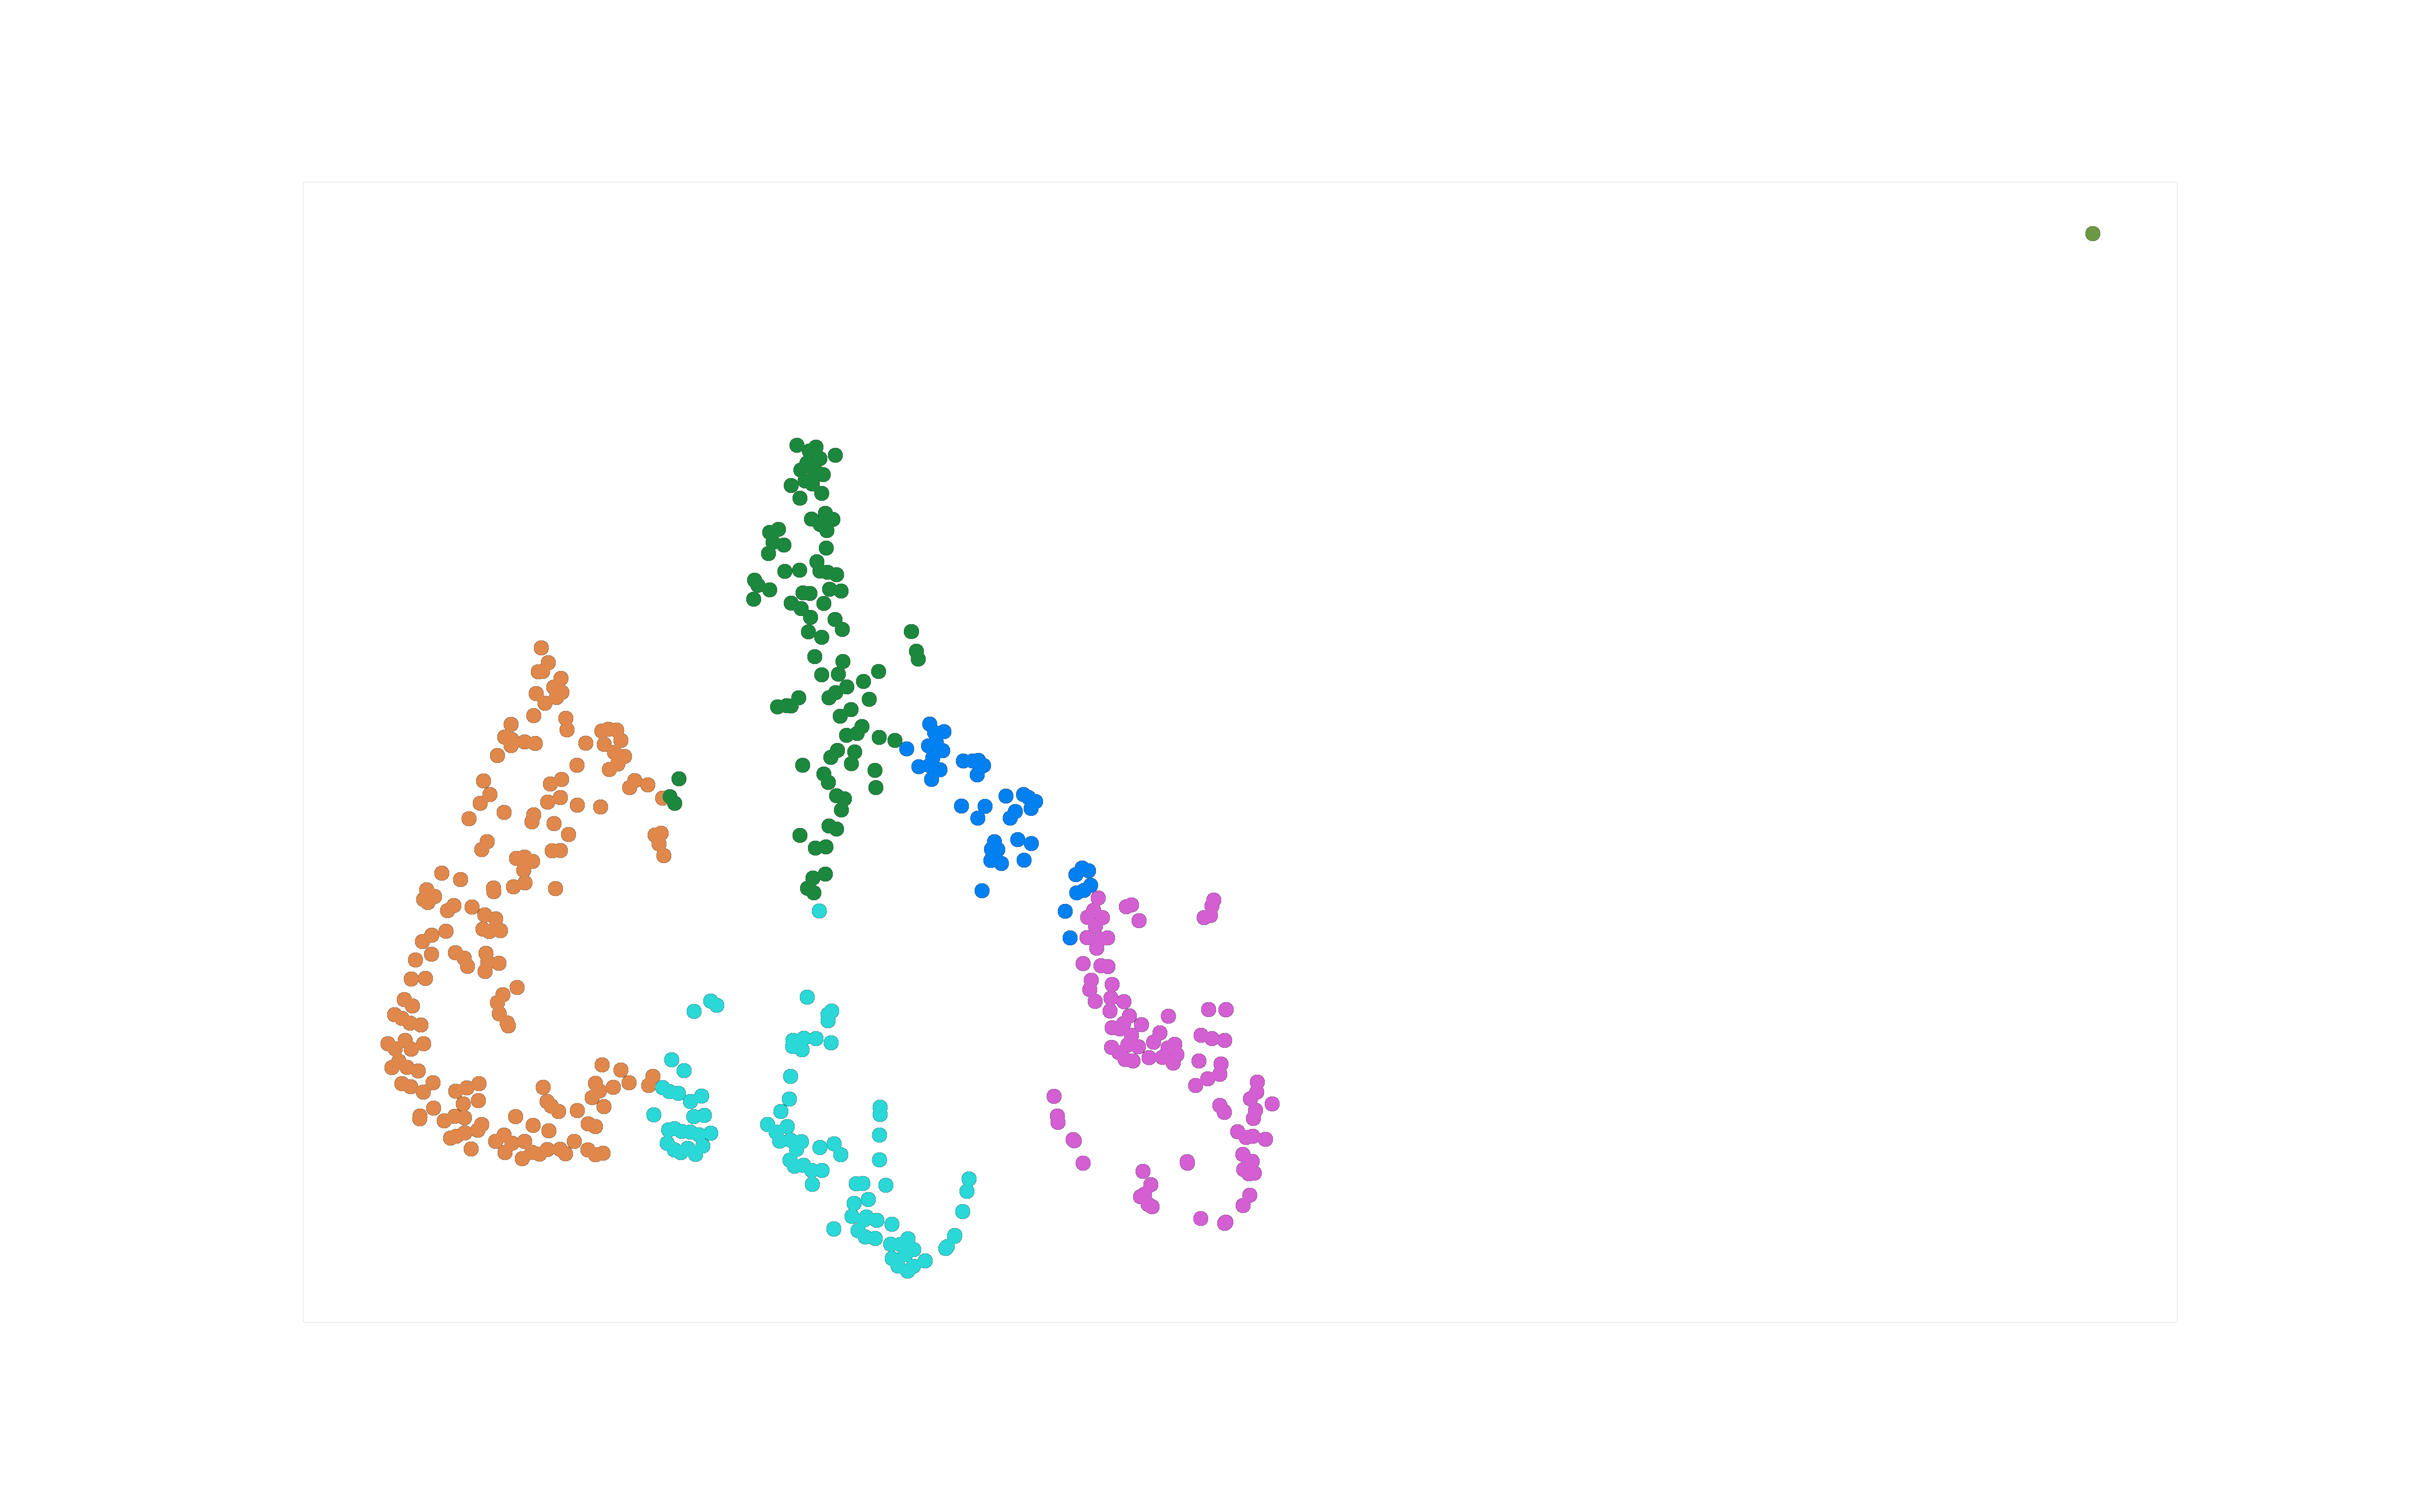
\includegraphics[scale=.3]{tsne_knn.png}
\subsubsection{DBSCAN}
To eliminate any possible outliers in the clustering, the embeddings were also fed into a DBSCAN clustering algorithm.  DBSCAN clustering is density based, and as such, it is extremely effective at grouping data points while leaving no outliers.  The visualization of the DBSCAN clustered data is below.\\[2mm]
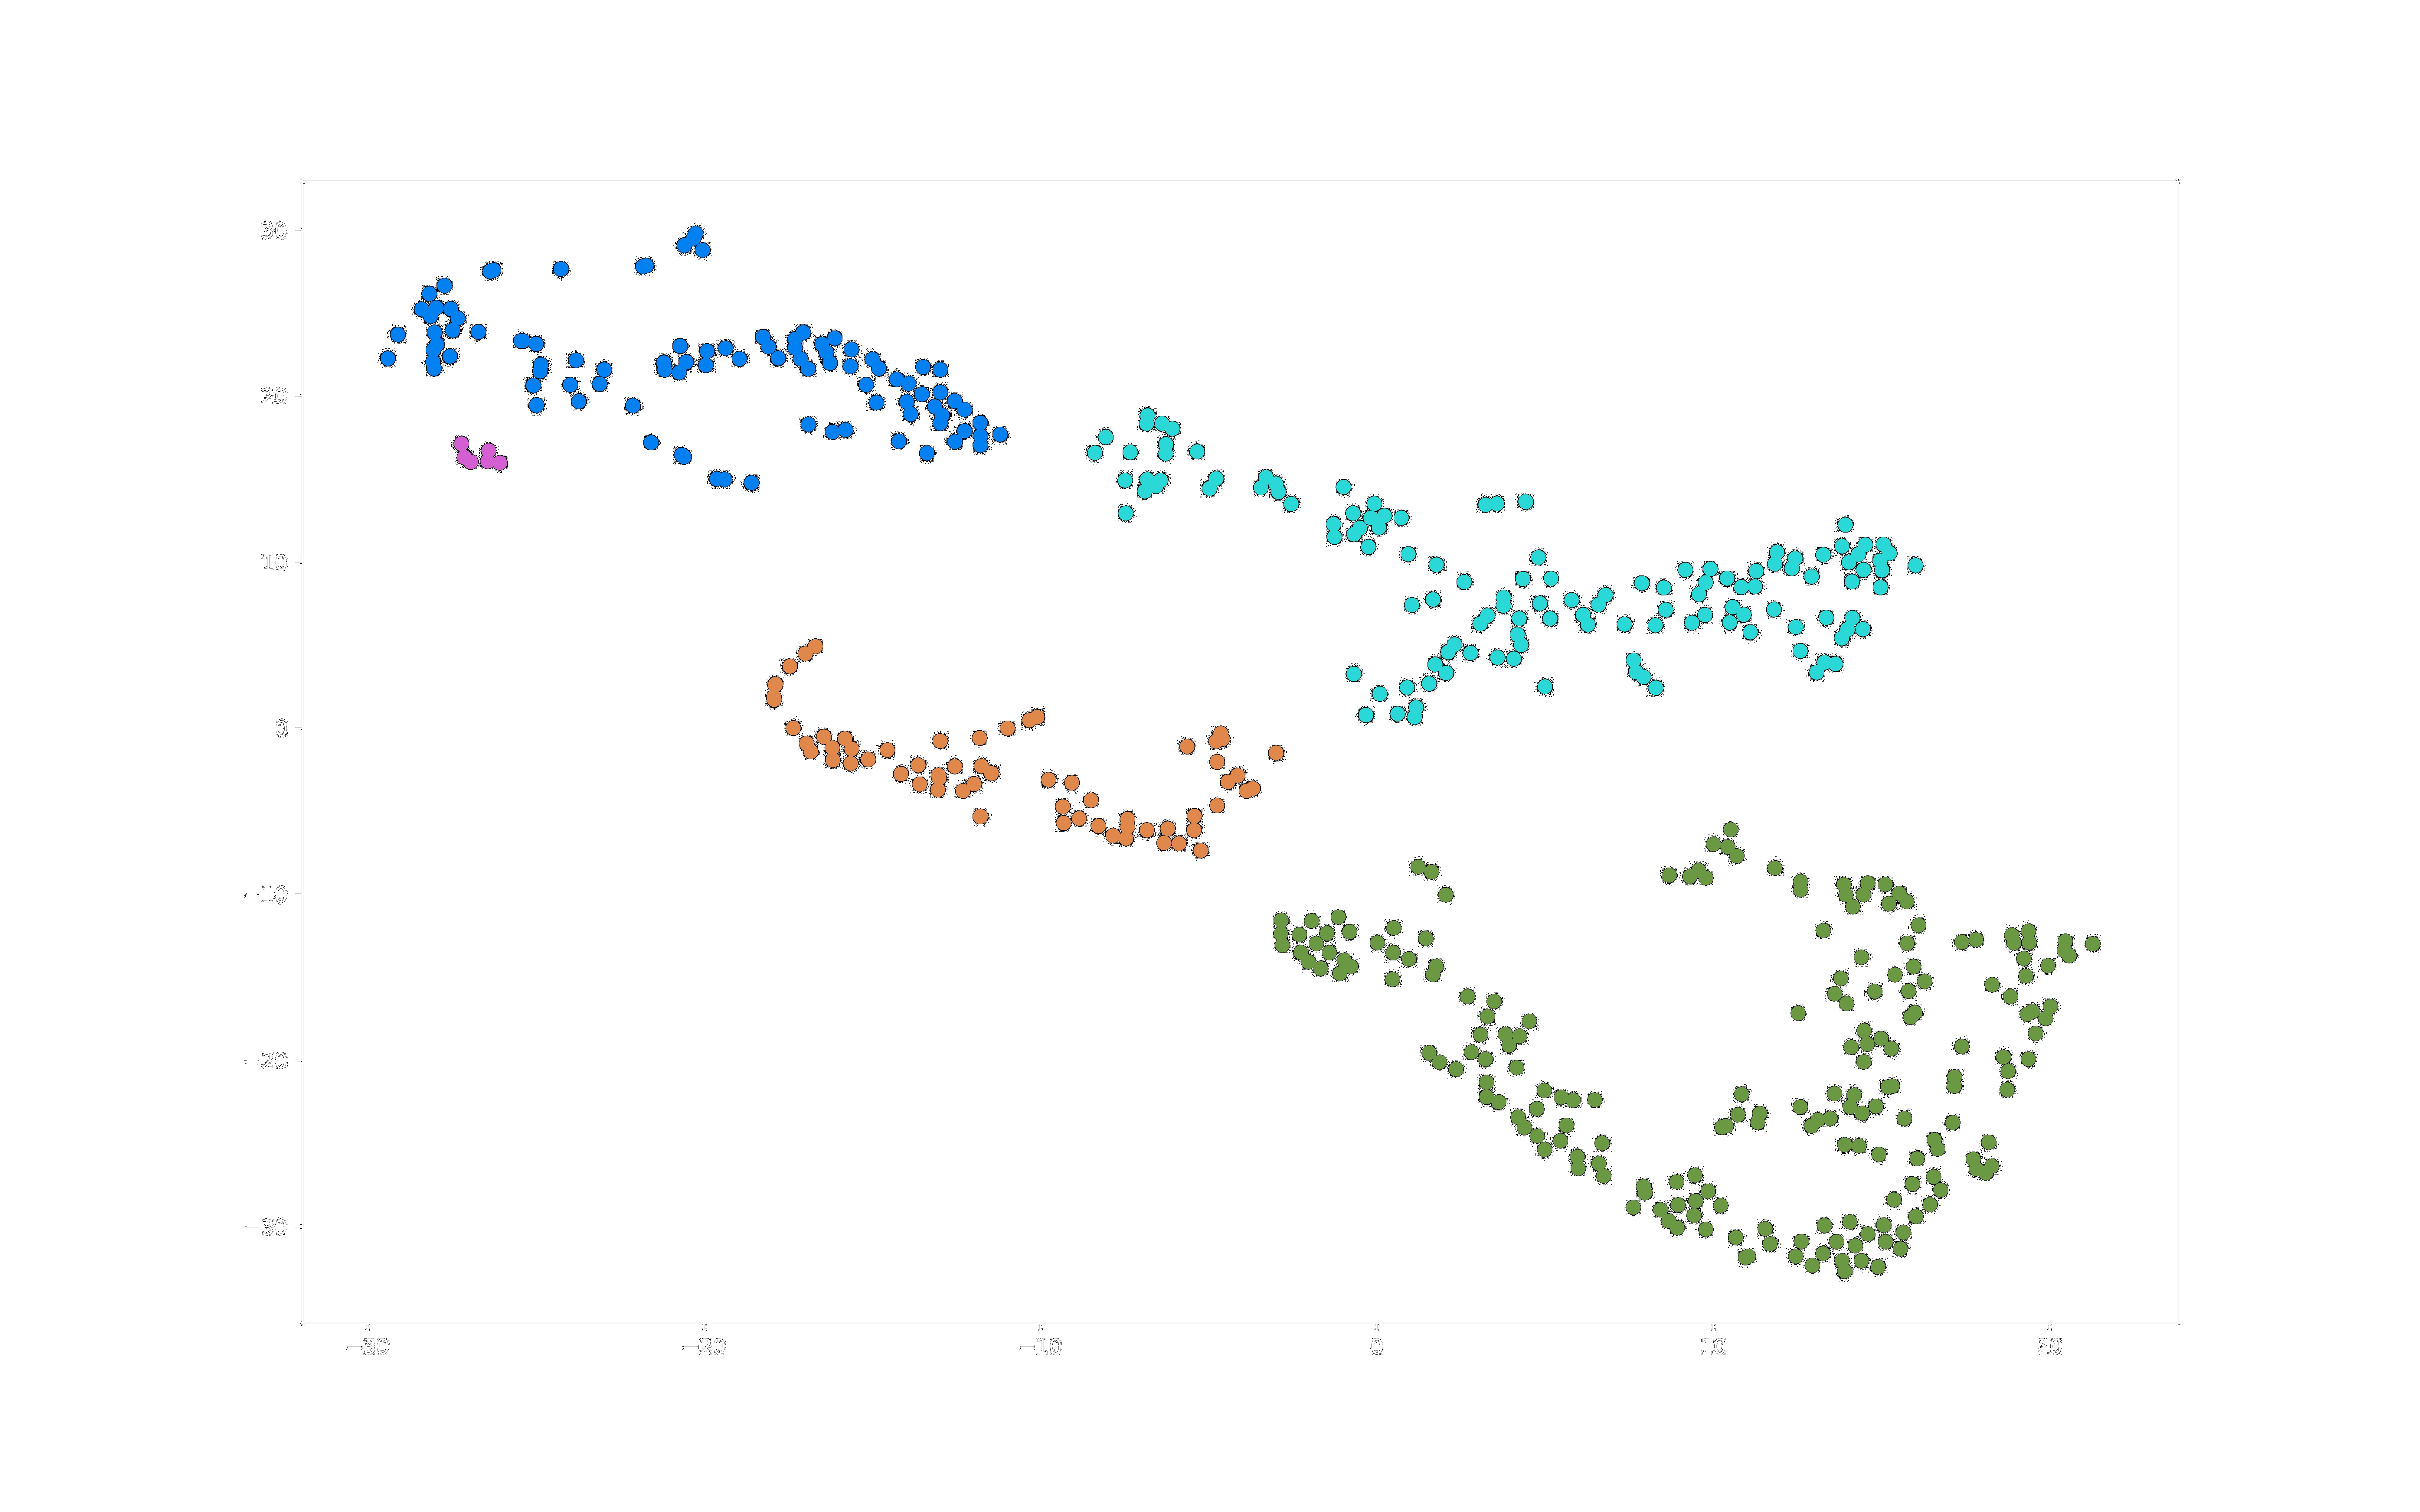
\includegraphics[scale=.3]{dbscan.png}
\np

\subsection{Regression Similarity}
For every pair of cryptocurrencies, a simple regression was computed.  First, the prices of each cryptocurrency were normalized from 0 to 1.  This was done to standardize the price axis to a common scale - some cryptocurrencies have a market value in the tens of thousands, while some others are worth hundredths of a cent.\\[2mm]
Next, a linear regression was run, and the $r^{2}$ was calculated.  Overall, this produces an $r^{2}$ for each pair of cryptocurrencies that represents how similar their price histories are.\\[2mm]
Below are some examples of the linear correlations found:\\
\begin{minipage}{0.45\textwidth}
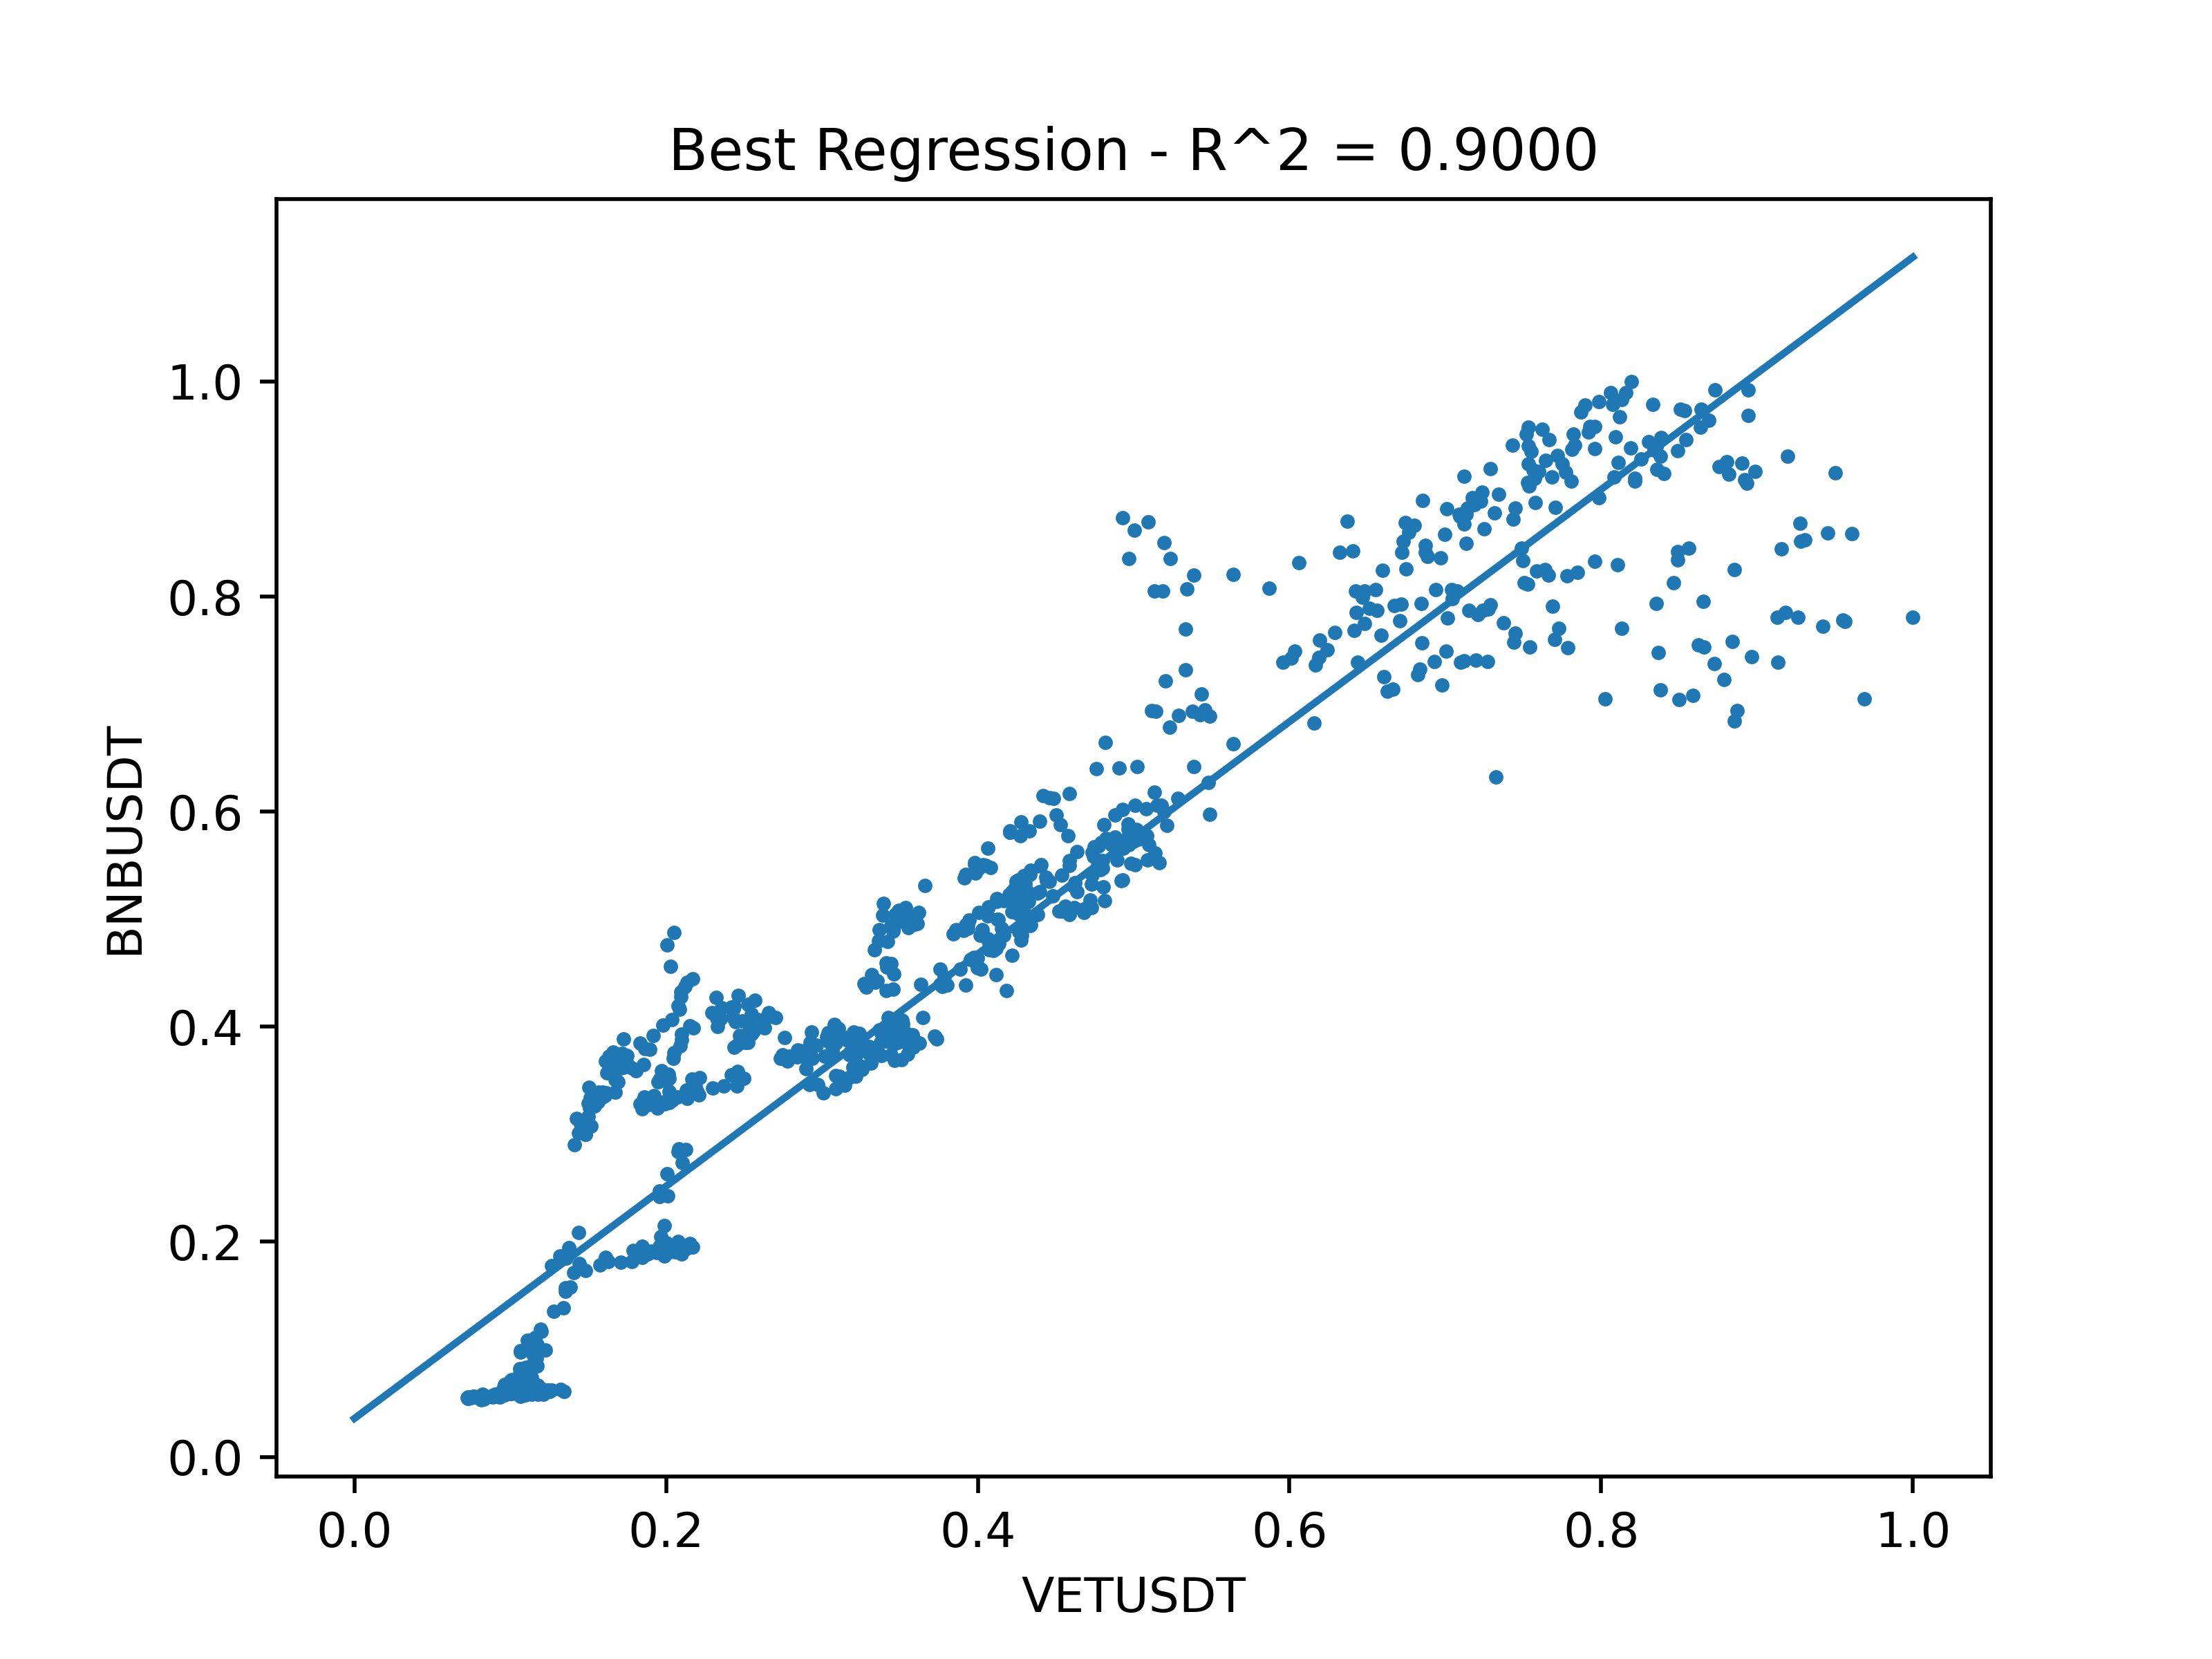
\includegraphics[scale=0.5]{best_reg.png}
\end{minipage}
\hfill
\begin{minipage}{0.45\textwidth}
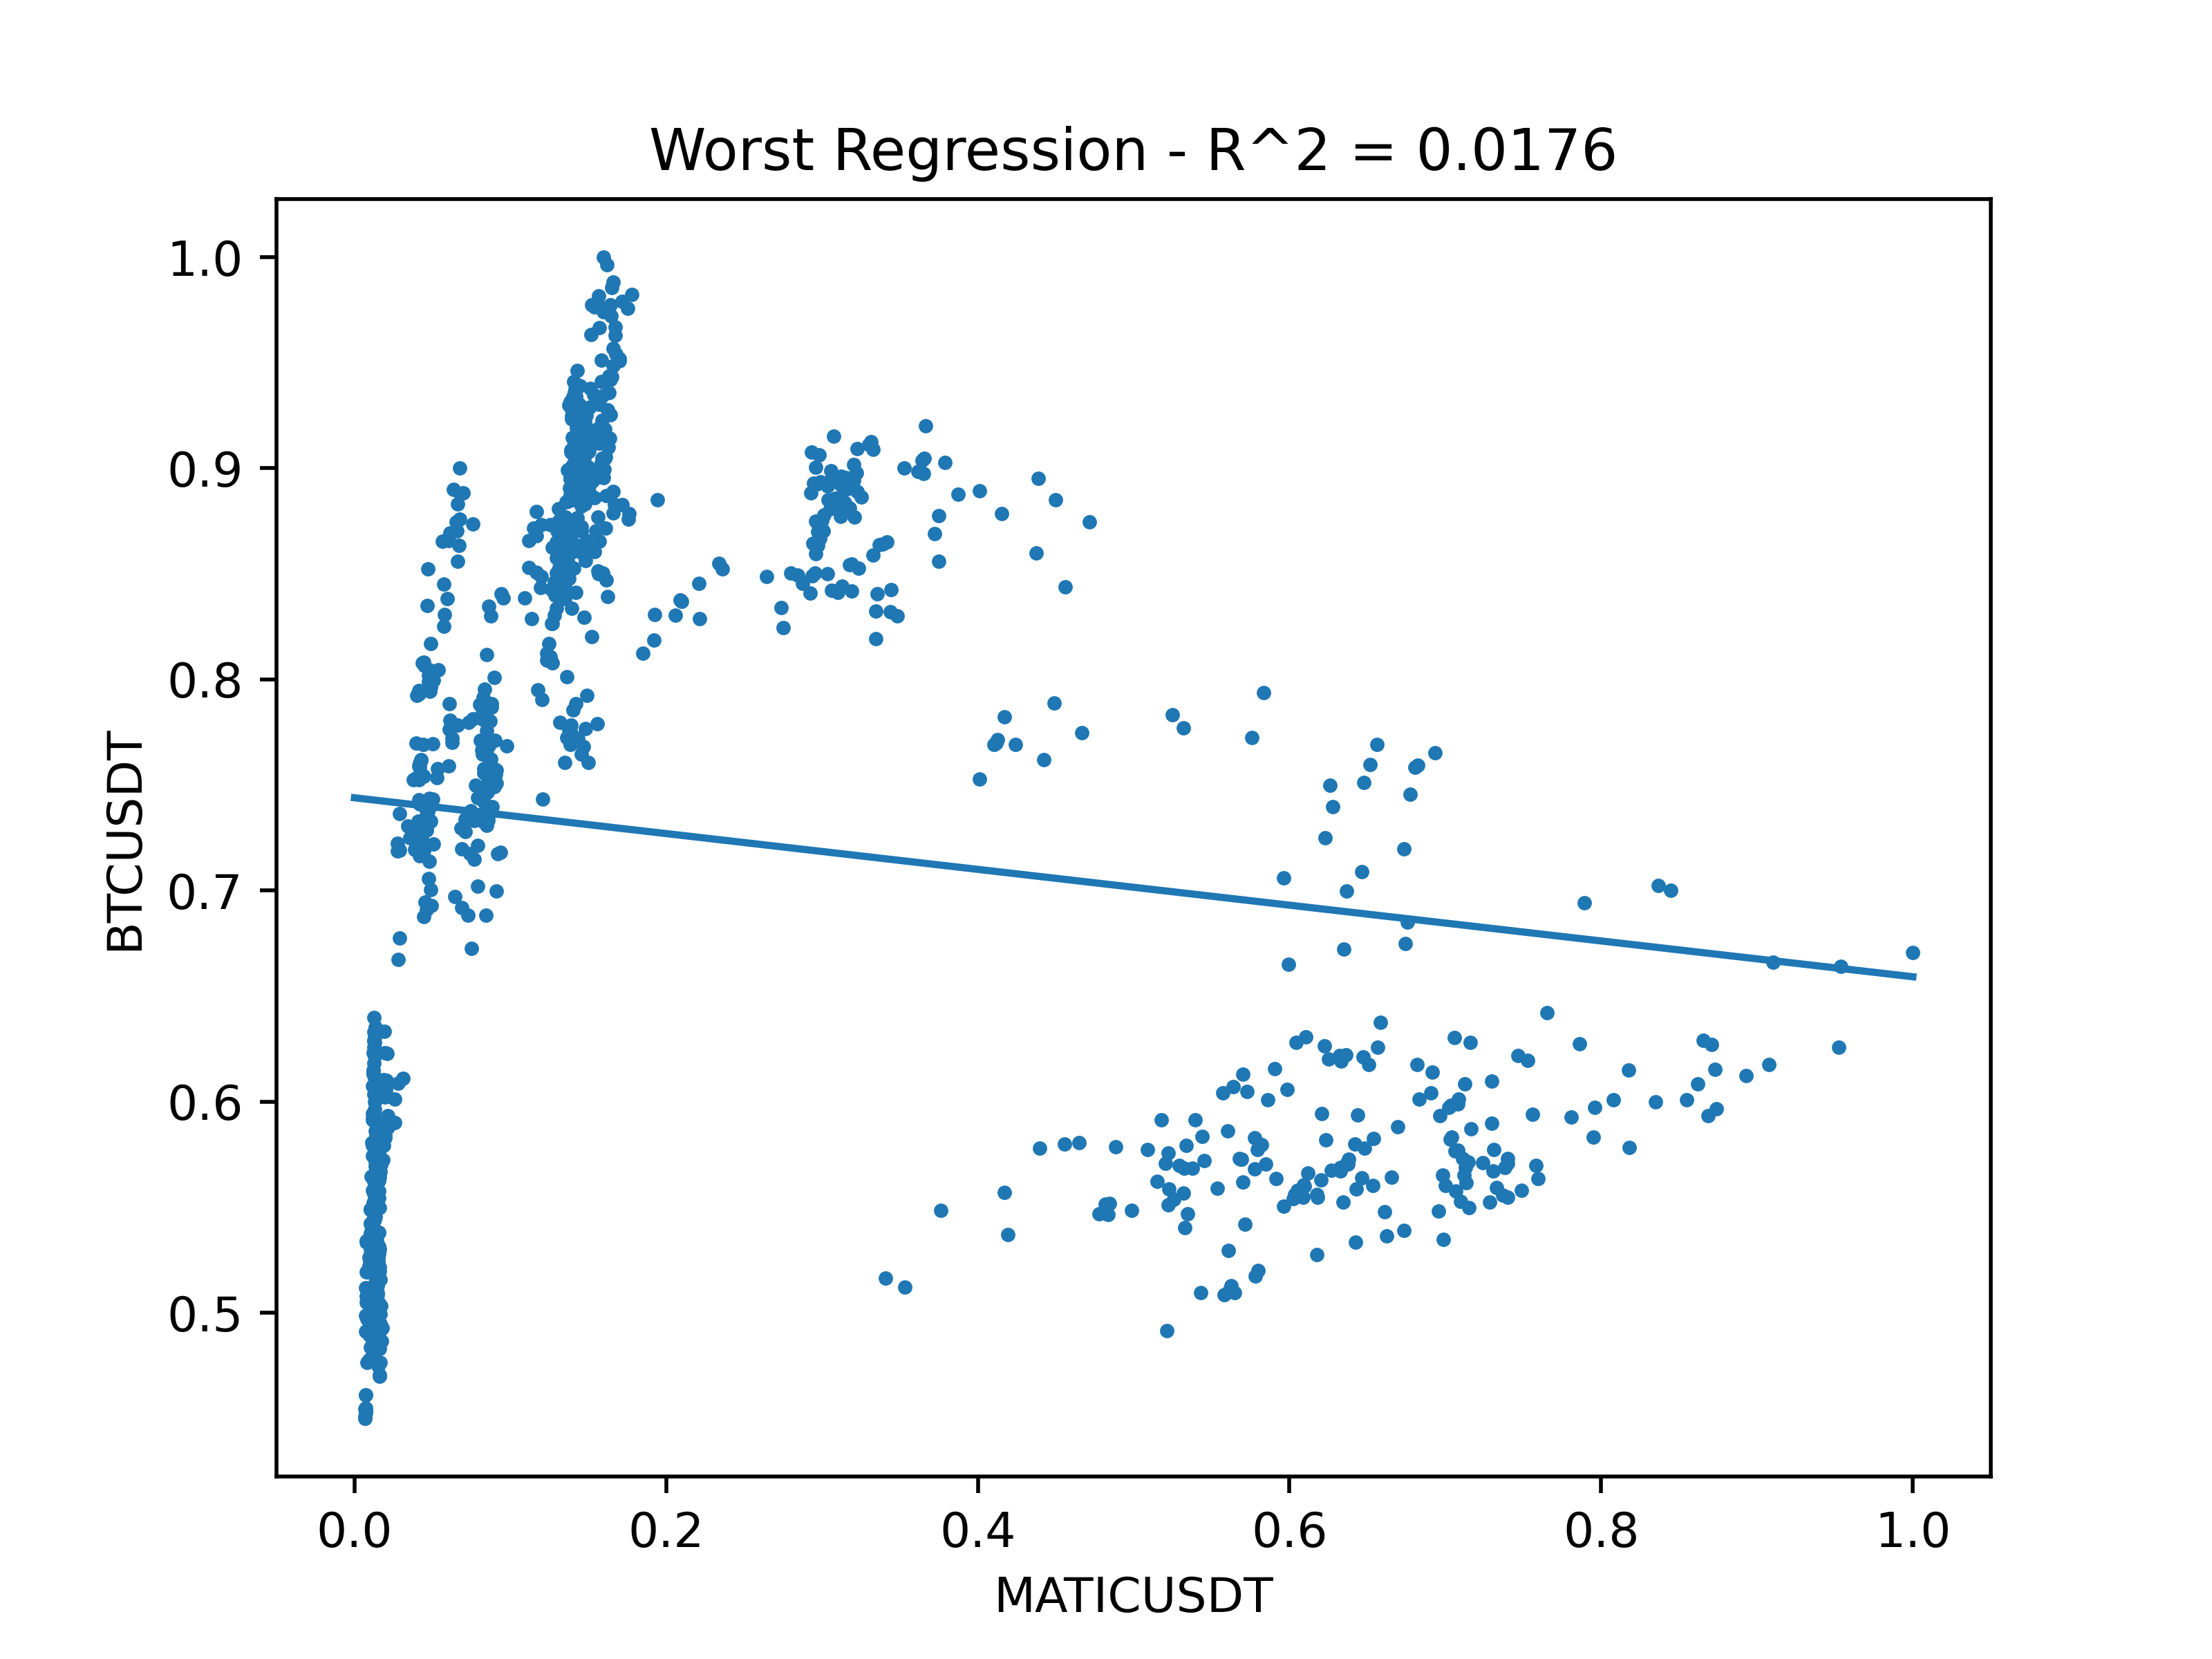
\includegraphics[scale=0.5]{worst_reg.png}
\end{minipage}\\[2mm]

\subsection{Correlation Prediction}
The goal of correlation prediction is to predict future correlation interaction between different pairs of cryptocurrencies, by looking at the past correlation data. Instead of using a traditional linear-regression / polynomial-fit SVM to make predictions on each possible pair, a graph-based neural network was utilized since the interaction between neighboring pairs is also a crucial piece of information\\[2mm]
The input to the model is a series of complete graphs, with each node representing a unique cryptocurrency asset, and the edges being the correlation index calculated using the Pearson’s Correlation Coefficient, for both closing price and trading volume. Each graph represents the state of the market at a specific unix timestamp. The model input is fed into multiple convolutional layers for it to learn the interaction between different pairs of cryptocurrencies as well as the temporal changes of the correlation.\\[2mm]
The model takes in the past 30 days of graphs (represented as an adjacency list) and predicts the next graph representing the correlation state of the next four hours. By reusing the predicted graphs as an input to the model we were able to produce a series of future correlation graphs at decreasing accuracy.\\[2mm]
The result of the correlation prediction is visualized by varying the color of the edges. The color spectrum we use is blue to magenta, which represents a correlation index of -1 to 1. Here are several frames of such predictions:\\[2mm]
\begin{minipage}{0.3\textwidth}
Hour 0:\\
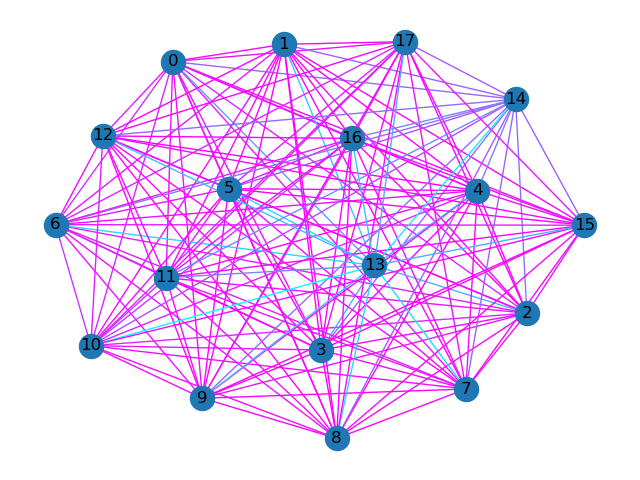
\includegraphics[scale=0.35]{../cor_images/p_800.png}\\
Hour 360:\\
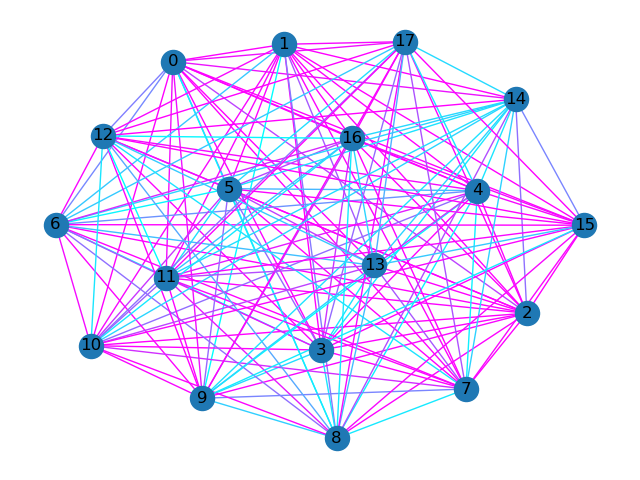
\includegraphics[scale=0.35]{../cor_images/p_890.png}
\end{minipage}
\hfill
\begin{minipage}{0.3\textwidth}
Hour 120:\\
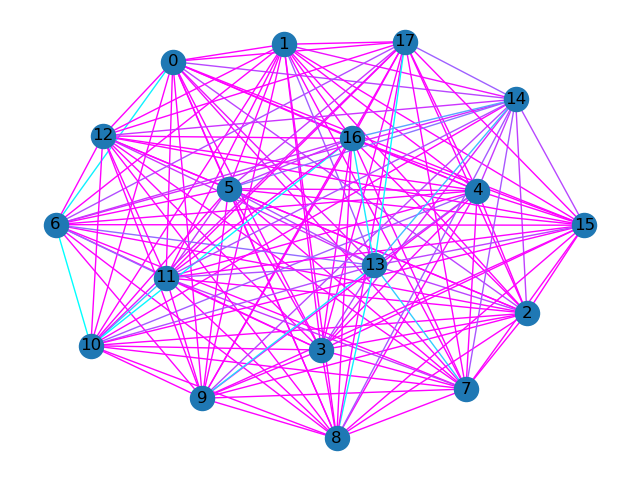
\includegraphics[scale=0.35]{../cor_images/p_830.png}\\
Hour 480:\\
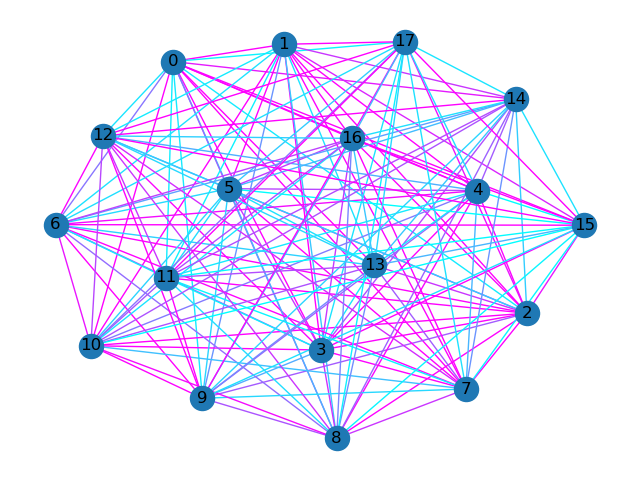
\includegraphics[scale=0.35]{../cor_images/p_920.png}
\end{minipage}
\hfill
\begin{minipage}{0.3\textwidth}
Hour 240:\\
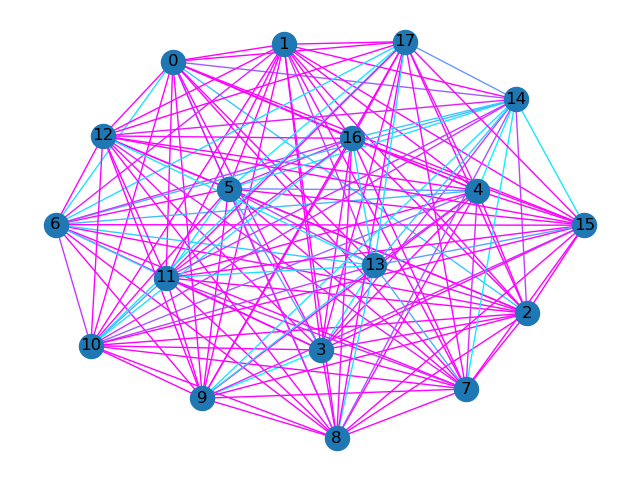
\includegraphics[scale=0.35]{../cor_images/p_860.png}\\
Hour 600:\\
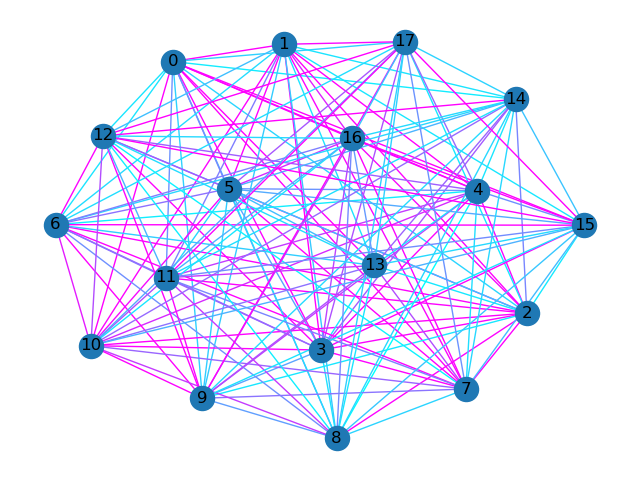
\includegraphics[scale=0.35]{../cor_images/p_950.png}
\end{minipage}\\[2mm]
The 3 frames above are the prediction of the state of closing price correlations between different cryptos in future timestamps. For the ease of viewing, the closing price correlation prediction was composed into a video (Video link: https://drive.google.com/file/d/16mhfgLrw0iKaZsb2u0Rs\_9Fx8uMXv2al/view?usp=sharing).\\[2mm]
An effective metric to evaluate the performance of this model has not yet been found, but for now the predictions within the first few days appear to be relatively reliable.

\subsection{Sentiment Analysis}
Sentiment analysis is a key part of real-time price prediction.  Large cryptocurrency price movements often stem from significant news, and sentiment analysis can be used to determine the general opinion of the public with regards to each cryptocurrency.\\[2mm]
Posts were scraped from Reddit (r/cryptocurrency), and the titles were fed through a pretrained BERT model.  This model was able to determine bullish/bearish/neutral sentiment with an accuracy of over 90\%.\\[2mm]
\np

\section{Method}
The backbone of the prediction model is a complete graph, where each node is a unique cryptocurrency, and each edge holds similarity data for each pair of cryptocurrencies, which includes K-means cluster ID, DBSCAN, cluster ID, linear regression $r^{2}$, etc.\\[2mm]
It is difficult to reasonably visualize a graph with multiple edge weights, so for the example graph below, only the weights for the linear regression are used:\\[2mm]
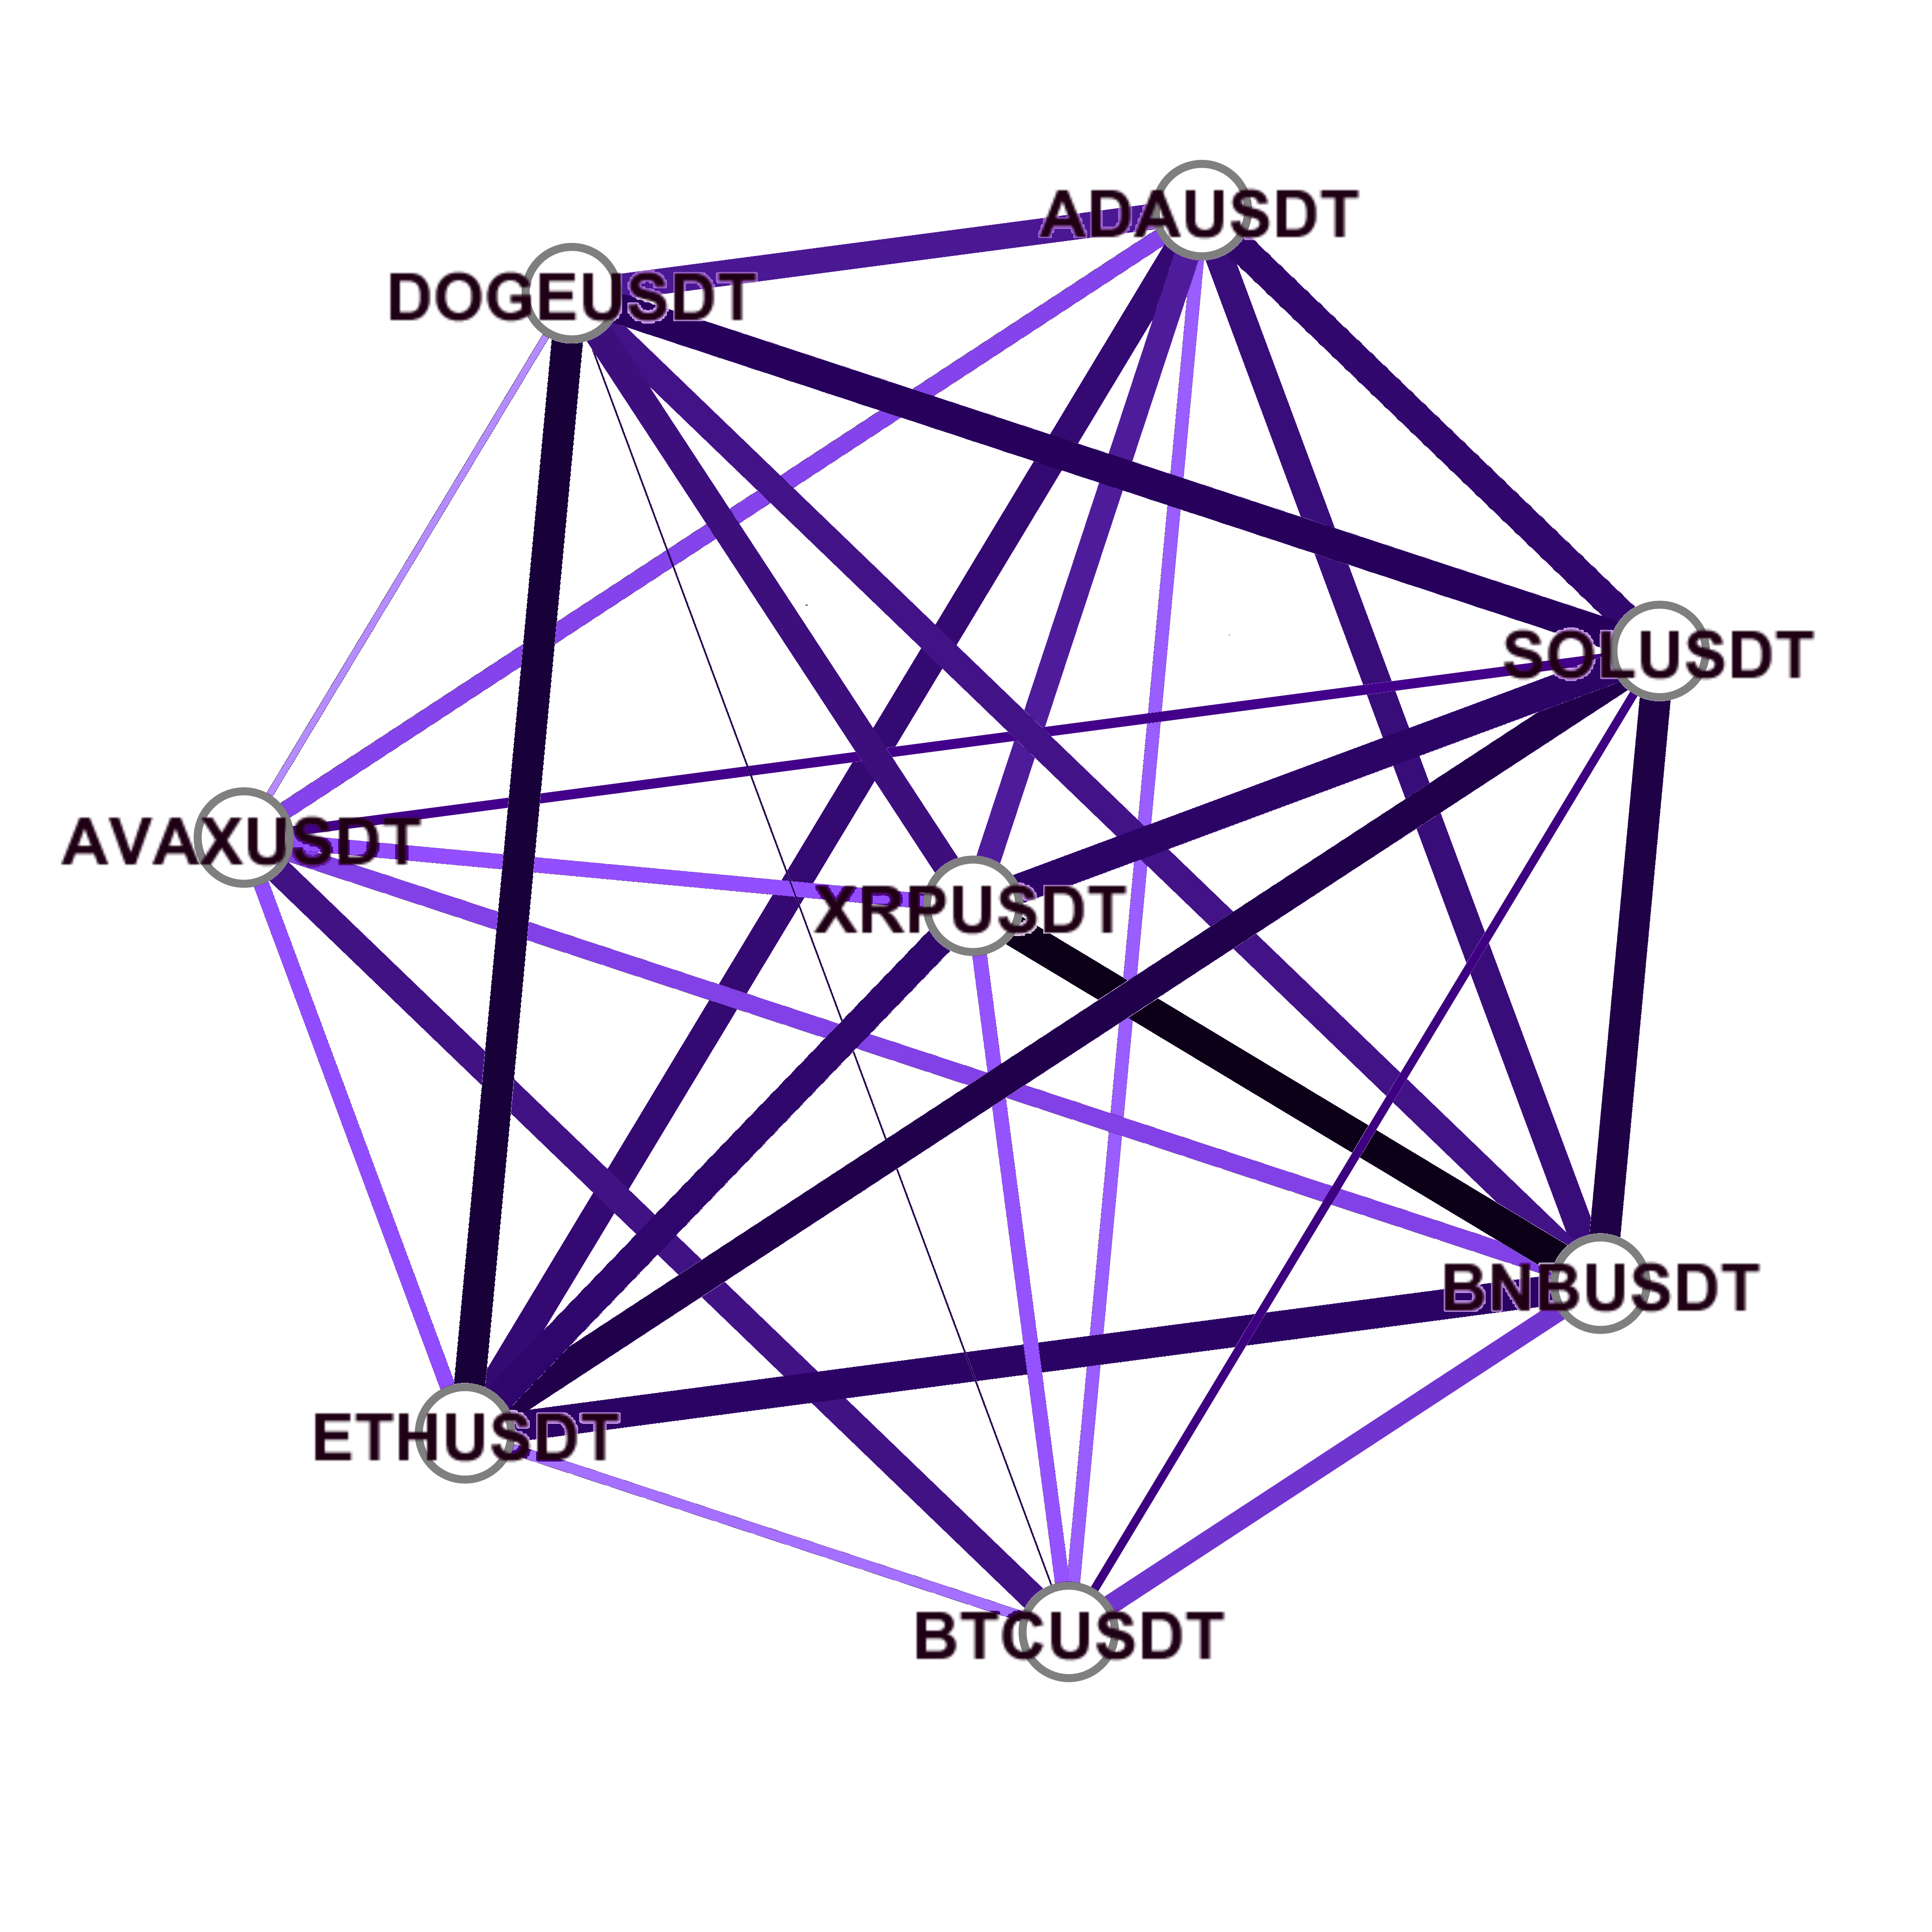
\includegraphics[width=8cm]{correlation_graph_small2.png}\\[2mm]
Given a cryptocurrency asset, the model finds the 10 most similar cryptocurrencies based on a weighted scoring system. The aggregate score is calculated using different clustering metrics (DBSCAN, K-means, etc.) as well as the linear regression $r^{2}$ on historical prices mentioned above. Since the clustering metrics are trained with metadata of the respective cryptocurrency asset (which is constant in the short-run) and linear regression on historical price, we are able to produce a similarity score that takes into consider of both static traits (ex: max-supply, market-cap) and quantitative price data.\\[2mm]


\section{Summary of Findings}
\subsection{Results}
An unbiased and quantitative evaluation metric for this model has not been found, but from extended testing, it was found that the resulting output of the similarity model agrees with the price correlation, and the actual price of the cryptos to some extent.\\[2mm]

The similarity score produced by the model is trivially correlated with previous price data, and for future price data, the model is able to accurately find cryptocurrencies that tend to move with each other.\\[2mm]

\subsection{Possible Confounding of Data}
Although the data and results show a strong positive correlation, it is likely that the similarities that were observed between cryptocurrencies are largely due to market-wide price movements.  More often than not, the entirety (or close to the entirety) of the cryptocurrency market moves together.  This leads to the price history of many cryptos appearing to be directly correlated with each other, when they are, in actuality, correlated with BTCUSDT, ETHUSDT, or another coin.\\[2mm]
In other words, the similarity metrics that were used may not be a good representation of possible similarities between cryptocurrencies, despite the observation of good performance.\\[2mm]


\section{Conclusion}
\subsection{Completed Goals}
Ultimately, the prediction and grouping of similar cryptocurrencies was implemented and appears to work relatively well.  Also completed is correlation prediction, sentiment analysis, and real-time scraping.  The completed work, however, was not analogous to the initial goals that were set at the beginning of the project.

\subsection{Incomplete Goals}
The largest unimplemented feature was real-time price prediction.  While piecing together a working real-time module, it became evident that it was quickly going out of scope of the assignment, as it had very little to do with graph mining and graphs in general.  It was extremely algorithm based, with data being stored in non-graph data structures.  Additionally, issues with the Twitter API, and fundamental 
flaws in the scraping logic led to real-time price prediction being dropped.\\[2mm]
A direct result of this was several unused, but functional modules that were intended to be used in real-time prediction.  This includes sentiment analysis using BERT, correlation prediction, and various custom technical indicators that were implemented.

\subsection{Future Work}
A clear next step would be to piece together the real-time price prediction.  This should theoretically be straightforward, as most of the fundamental components of the model are already completed.  The primary focus would be on working around the core issues that were encountered, such as the Twitter API only storing 7 days of prior tweets, and the delay between news, price movement, and when the data could be scraped and processed.

\np
\section{Sample Output}
Below is an example use of the program.\\[2mm]
\begin{verbatim}
Enter a ticker for similar cryptocurrencies: BTCUSDT
Top 10 similar cryptocurrencies:
        01: NEARUSDT     similarity: 0.928039
        02: DOTUSDT      similarity: 0.910973
        03: ATOMUSDT     similarity: 0.890866
        04: EGLDUSDT     similarity: 0.886348
        05: SANDUSDT     similarity: 0.880285
        06: LUNAUSDT     similarity: 0.877113
        07: BATUSDT      similarity: 0.826980
        08: XTZUSDT      similarity: 0.822819
        09: AVAXUSDT     similarity: 0.818994
        10: DASHUSDT     similarity: 0.797945

Enter a ticker for similar cryptocurrencies: NEARUSDT
Top 10 similar cryptocurrencies:
        01: DOTUSDT      similarity: 0.953060
        02: SANDUSDT     similarity: 0.939675
        03: LUNAUSDT     similarity: 0.933701
        04: BTCUSDT      similarity: 0.928039
        05: ATOMUSDT     similarity: 0.886720
        06: ENJUSDT      similarity: 0.883375
        07: BATUSDT      similarity: 0.883180
        08: EGLDUSDT     similarity: 0.875387
        09: UNIUSDT      similarity: 0.846779
        10: FTTUSDT      similarity: 0.841460

Enter a ticker for similar cryptocurrencies: ETHUSDT
Top 10 similar cryptocurrencies:
        01: MKRUSDT      similarity: 0.976515
        02: WAVESUSDT    similarity: 0.962074
        03: RUNEUSDT     similarity: 0.954988
        04: EOSUSDT      similarity: 0.949072
        05: ETCUSDT      similarity: 0.930652
        06: SOLUSDT      similarity: 0.926456
        07: BCHUSDT      similarity: 0.924530
        08: XMRUSDT      similarity: 0.904530
        09: BNBUSDT      similarity: 0.899182
        10: NEOUSDT      similarity: 0.897319

Enter a ticker for similar cryptocurrencies: ADAUSDT
Top 10 similar cryptocurrencies:
        01: MATICUSDT    similarity: 0.814132
        02: ALGOUSDT     similarity: 0.746764
        03: DOGEUSDT     similarity: 0.564805
        04: XRPUSDT      similarity: 0.546123
        05: HBARUSDT     similarity: 0.540680
        06: VETUSDT      similarity: 0.533386
        07: ONEUSDT      similarity: 0.519367
        08: XLMUSDT      similarity: 0.519099
        09: TRXUSDT      similarity: 0.513903
        10: IOTXUSDT     similarity: 0.508165

Enter a ticker for similar cryptocurrencies: NOTACRYPTO
Ticker is not in graph.

Enter a ticker for similar cryptocurrencies: exit
\end{verbatim}
\end{document}